\documentclass[a4paper,11pt] {article}
\usepackage{graphicx}
\usepackage{amssymb, amsmath, amsthm}
\usepackage{setspace}
\usepackage{amsfonts}

%-----------Margin, Linespread, Spacing-----------%
\usepackage[letterpaper, margin=1.3in]{geometry}
\usepackage[letterpaper]{geometry}
\linespread{1}
%-------------------------------------------------%

%-----------Define header and footnotes-----------
\usepackage{fancyhdr}               % Header and footnotes
\pagestyle{fancy}
\lhead{\bfseries \scriptsize CQF}
\chead{\bfseries \scriptsize Module 4 Solution}
\rhead{\bfseries \scriptsize Ran Zhao}
\renewcommand{\headrulewidth}{0.4pt}
%-------------------------------------------------%

%---------------------Listings--------------------%
\usepackage{listings}
\usepackage{color}
\definecolor{dkgreen}{rgb}{0,0.6,0}
\definecolor{gray}{rgb}{0.5,0.5,0.5}
\definecolor{mauve}{rgb}{0.58,0,0.82}
\lstset{ %
  language=Octave,                % the language of the code
  basicstyle=\footnotesize,           % the size of the fonts that are used for the code
  numbers=left,                   % where to put the line-numbers
  numberstyle=\tiny\color{gray},  % the style that is used for the line-numbers
  stepnumber=2,                   % the step between two line-numbers. If it's 1, each line
                                  % will be numbered
  numbersep=5pt,                  % how far the line-numbers are from the code
  backgroundcolor=\color{white},      % choose the background color. You must add \usepackage{color}
  showspaces=false,               % show spaces adding particular underscores
  showstringspaces=false,         % underline spaces within strings
  showtabs=false,                 % show tabs within strings adding particular underscores
  frame=single,                   % adds a frame around the code
  rulecolor=\color{black},        % if not set, the frame-color may be changed on line-breaks within not-black text (e.g. commens (green here))
  tabsize=2,                      % sets default tabsize to 2 spaces
  captionpos=b,                   % sets the caption-position to bottom
  breaklines=true,                % sets automatic line breaking
  breakatwhitespace=false,        % sets if automatic breaks should only happen at whitespace
  title=\lstname,                   % show the filename of files included with \lstinputlisting;
                                  % also try caption instead of title
  keywordstyle=\color{blue},          % keyword style
  commentstyle=\color{dkgreen},       % comment style
  stringstyle=\color{mauve},         % string literal style
  escapeinside={\%*}{*)},            % if you want to add LaTeX within your code
  morekeywords={*,...}               % if you want to add more keywords to the set
}
%-------------------------------------------------%

%----------------Title, Author, Dates-------------
\author{Ran Zhao}
\title{CQF Module 4 Exercise Solution}
\date{}
\begin{document}
\maketitle
%--------------------------------------------------


\textcolor{blue}{\bf 1 } The zero coupon bonds satisfy
\begin{equation} \label{eqn::zero_bond}
\frac{\partial Z}{\partial t} + \frac{1}{2} \omega(r,t)^2 \frac{\partial^2 Z}{\partial r^2} + [u(r,t)-\lambda(r,t)\omega(r,t)] \frac{\partial Z}{\partial r} - rZ = 0
\end{equation}

As time being close to the maturity ($T-t\rightarrow 0$), expand the zero coupon bond with the form
\begin{equation} \label{eqn::zero_bond_expansion}
Z\sim 1 + a(r)(T-t) + b(r)(T-t)^2 + \ldots
\end{equation}

substitute $Z$ in Equation~\ref{eqn::zero_bond_expansion} into Equation~\ref{eqn::zero_bond}, and equating powers of $(T-t)$ yields
$$
Z(r,t;T)\sim 1 -r(T-t) + \frac{1}{2}(T-t)^2(r^2-u+\lambda\omega) + \ldots \qquad \textrm{as } t\rightarrow T
$$

So the shape of the yield curve near the short end becomes
$$
-\frac{\ln Z}{T-t} \sim r + \frac{1}{2}(u-\lambda\omega)(T-t) + \ldots \qquad \textrm{as } t\rightarrow T
$$

In Vasicek model, the risk-neutral spot rate take the form
$$
dr = (\eta-\gamma r) dt + \sqrt{\beta} dX
$$

and we have
$$
u-\lambda\omega = \eta-\gamma r
$$

Therefore, for the Vasicek model with one month Libor, we find
$$
r_L \sim r + \frac{1}{2}(\eta-\gamma r) \frac{1}{12}
$$

Finally, a floorlet cashflow has approximate value
$$
\max(r_f - r_L, 0) \sim \max\left(r_f - r - \frac{1}{24} (\eta-\gamma r), 0\right)
$$
as claimed.

\bigskip

\textcolor{blue}{\bf 2 } The Black-Derman \& Toy short-rate model is
\begin{equation} \label{eqn::BDT}
d(\log r) = \left( \theta(t) + \frac{d(\log\sigma(t))}{dt} \log r \right) dt + \sigma(t) dW
\end{equation}

Let $f(x) = \exp x$ and $X = \log r$. Apply It$\hat{o}$'s Lemma on $f(X)$ we obtain
$$
d(f(X)) = \frac{\partial f}{\partial X} dX + \frac{1}{2} \frac{\partial f^2}{\partial^2 X} dX^2
$$

where $\partial f / \partial X = \exp(X) = r$ and $\partial f^2 / \partial^2 X = \exp(X) = r$. Given $dX$ from Equation~\ref{eqn::BDT}, we then have
\begin{eqnarray*}
d(f(X)) &=& dr =  \frac{\partial f}{\partial X} dX + \frac{1}{2} \frac{\partial f^2}{\partial^2 X} dX^2 \\
        &=& r(t)\left( \theta(t) + \frac{d(\log\sigma(t))}{dt} \log r \right) dt + \sigma(t)r(t) dW + \frac{1}{2}\sigma^2(t) dt \\
        &=& r(t)\left( \theta(t) + \frac{d(\log\sigma(t))}{dt} \log r + \frac{1}{2} \sigma^2(t) \right) dt + \sigma(t)r(t) dW
\end{eqnarray*}

Using the notation of
$$
dr = A(r,t)dt + B(r,t)dW
$$

yields
$$
\left\{
  \begin{array}{ccl}
    A(r,t) & = & r(t)\left( \theta(t) + \frac{d(\log\sigma(t))}{dt} \log r + \frac{1}{2} \sigma^2(t) \right) \\
    B(r,t) & = & \sigma(t)r(t) \\
  \end{array}
\right.
$$

The terminal condition, $Z(r,T;T)=1$, must hold for all $r$, and this implies that $A(T,T)=B(T,T)=0$.

\bigskip

\textcolor{blue}{\bf 3 } With model specification
$$
dr = [\eta(t)-\gamma r] dt + c dW
$$
where $\eta(t)$ is an arbitrary function of time $t$ and $\gamma$ and $c$ are constants. The partial differential
equation for the zero coupon bond price becomes
\begin{equation} \label{eqn::bond_hw}
\frac{\partial Z}{\partial t} + [\eta(t)-\gamma r]\frac{\partial Z}{\partial r} + \frac{1}{2}c^2 \frac{\partial^2 Z}{\partial r^2} = rZ
\end{equation}

Initially guess and subsequently verify that the solution has the form
$$
Z(r,t;T) = \exp(A(t;T)-rB(t;T))
$$
for some nonrandom functions $A(t;T)$ and $B(t;T)$ to be determined. Furthermore,
\begin{eqnarray*}
\frac{\partial Z}{\partial t}       &=& \left[\frac{\partial A(t,T)}{\partial t} - r\frac{\partial B(t,T)}{\partial t}\right]Z(r,t;T) \\
\frac{\partial Z}{\partial r}       &=& -B(t,T)Z(r,t;T) \\
\frac{\partial^2 Z}{\partial r^2}   &=& B(t,T)^2 Z(r,t;T)
\end{eqnarray*}

Substitution into the partial differential equation \ref{eqn::bond_hw} gives
\begin{equation} \label{eqn::eqn_bond_price}
\left[ \left( - \frac{\partial B(t,T)}{\partial t} + \gamma B(t,T) - 1 \right)r  \right. \\
+  \left. \frac{\partial A(t,T)}{\partial t}-\eta(t)B(t,T) +  \frac{1}{2}c^2 B(t,T)^2 \right]Z(r,t;T) = 0
\end{equation}

This equation must hold for all $r$, therefore the term that multiplies $r$ in this equation must be zero. Otherwise, changing the value of $r$ would change the value of the left-hand side of equation \ref{eqn::eqn_bond_price}, and hence it could not always be equal to zero. This gives us an ordinary differential equation in $t$ as
\begin{equation} \label{eqn::B_dyn}
\frac{\partial B(t,T)}{\partial t} = \gamma B(t,T) - 1
\end{equation}

Setting the term \ref{eqn::B_dyn} to zero in equation \ref{eqn::eqn_bond_price}, we have
\begin{equation} \label{eqn::A_dyn}
\frac{\partial A(t,T)}{\partial t} = \eta(t)B(t,T) -  \frac{1}{2}c^2 B(t,T)^2
\end{equation}

From the equation \ref{eqn::B_dyn}, it is not hard to solve
\begin{eqnarray*}
\frac{\partial B(t,T)}{\partial t} &=& \gamma B(t,T) - 1 \\
\frac{1}{\gamma} \frac{d (\gamma B(t,T) -1)}{\gamma B(t,T) -1} &=& d\tau \\
\frac{1}{\gamma} \int_t^T \frac{d (\gamma B(t,T) -1)}{\gamma B(t,T) -1} &=& \int_t^T d\tau \\
\frac{1}{\gamma} \log(\gamma B(t,T)-1) &=& - (T-t) \\
B(t,T) &=& \frac{1}{\gamma} \left( 1 - e^{-\gamma (T-t)} \right)
\end{eqnarray*}

Substitution the solution of $B(t,T)$ into \ref{eqn::A_dyn} yields
\begin{eqnarray*}
A(t,T) &=& - \left[ \int_t^T \eta(\tau)B(\tau,T) -  \frac{1}{2}c^2 B(\tau,T)^2 \right] d\tau \\
       &=& - \int_t^T \eta(\tau)B(\tau,T)d\tau + \frac{1}{2}c^2 \int_t^T \frac{1}{\gamma} \left( 1 - e^{-\gamma (T-t)} \right)^2 d\tau \\
       &=&  \int_t^T \eta(\tau)B(\tau,T)d\tau + \frac{c^2}{2\gamma^2} \left( (T-t) + \frac{2}{\gamma} e^{-\gamma(T-t)} -\frac{1}{2\gamma}e^{-2\gamma(T-t)} -\frac{3}{2\gamma} \right)
\end{eqnarray*}

And we solved $A(t,T)$ and $B(t,T)$ as claimed.

\bigskip

\textcolor{blue}{\bf 4 } Given the process
$$
dU_t = -\gamma U_t dt + \sigma dW_t
$$

we have
\begin{eqnarray*}
d(e^{\gamma }U_t) &=& \gamma e^{\gamma t} U_t dt + e^{\gamma t} d U_t \\
                  &=& \gamma e^{\gamma t} U_t dt - \gamma e^{\gamma t} U_t dt +  \sigma e^{\gamma t} dW_t \\
                  &=& \sigma e^{\gamma t} dW_t \\
e^{\gamma t} U_t  &=& U_0 + \sigma \int_{0}^{t}e^{\gamma s} dW_s \\
                  &=& u + \sigma \int_{0}^{t}e^{\gamma s} dW_s \\
U_t               &=& ue^{-\gamma t} + \sigma \int_0^t e^{-\gamma (t-s)} dW_s
\end{eqnarray*}

Then the moments of $U_t$ should be
\begin{eqnarray*}
\mathbb{E}[U_t] &=&  \mathbb{E}[ue^{-\gamma t}] + \mathbb{E}[\sigma \int_0^t e^{-\gamma (t-s)} dW_s] \\
                &=&  ue^{-\gamma t}  \\
\mathbb{V}[U_t] &=&  \mathbb{E}\left[ \sigma^2 \left( \int_0^t e^{-\gamma(t-s)}dW_s \right)^2 \right]  \\
                &=&  \sigma^2 \int_0^t e^{-2\gamma(t-s)} ds \\
                &=&  \frac{\sigma^2}{2\gamma} (1-e^{-2\gamma t})
\end{eqnarray*}

\bigskip

\textcolor{blue}{\bf 5 } The HJM framework is to model the evolution of the forward curve. Using the spreadsheet tool provided in the lecture, I perform the caplet option pricing in the HJM model. Generally, the price of caplet option written on 6M LIBOR with forward start date in six months from today is
$$
DF_{OIS}(0,1) \times \max(L(0;0.5,1)-K,0) \times \tau \times N
$$

In the spreadsheet, each calculation provides a pricing of Caplet with given parameters. I wrote a VBA code to perform the refreshing of the spreadsheet for many times, and each refresh generates a new scenario with recalculation on the Caplet. As shown in Figure~\ref{fig::scr_excel}, the button-click will populate 1,000 scenarios, with the annualized forward rate and corresponding Caplet price in each path.

\begin{center}
\begin{figure}
  \centering
  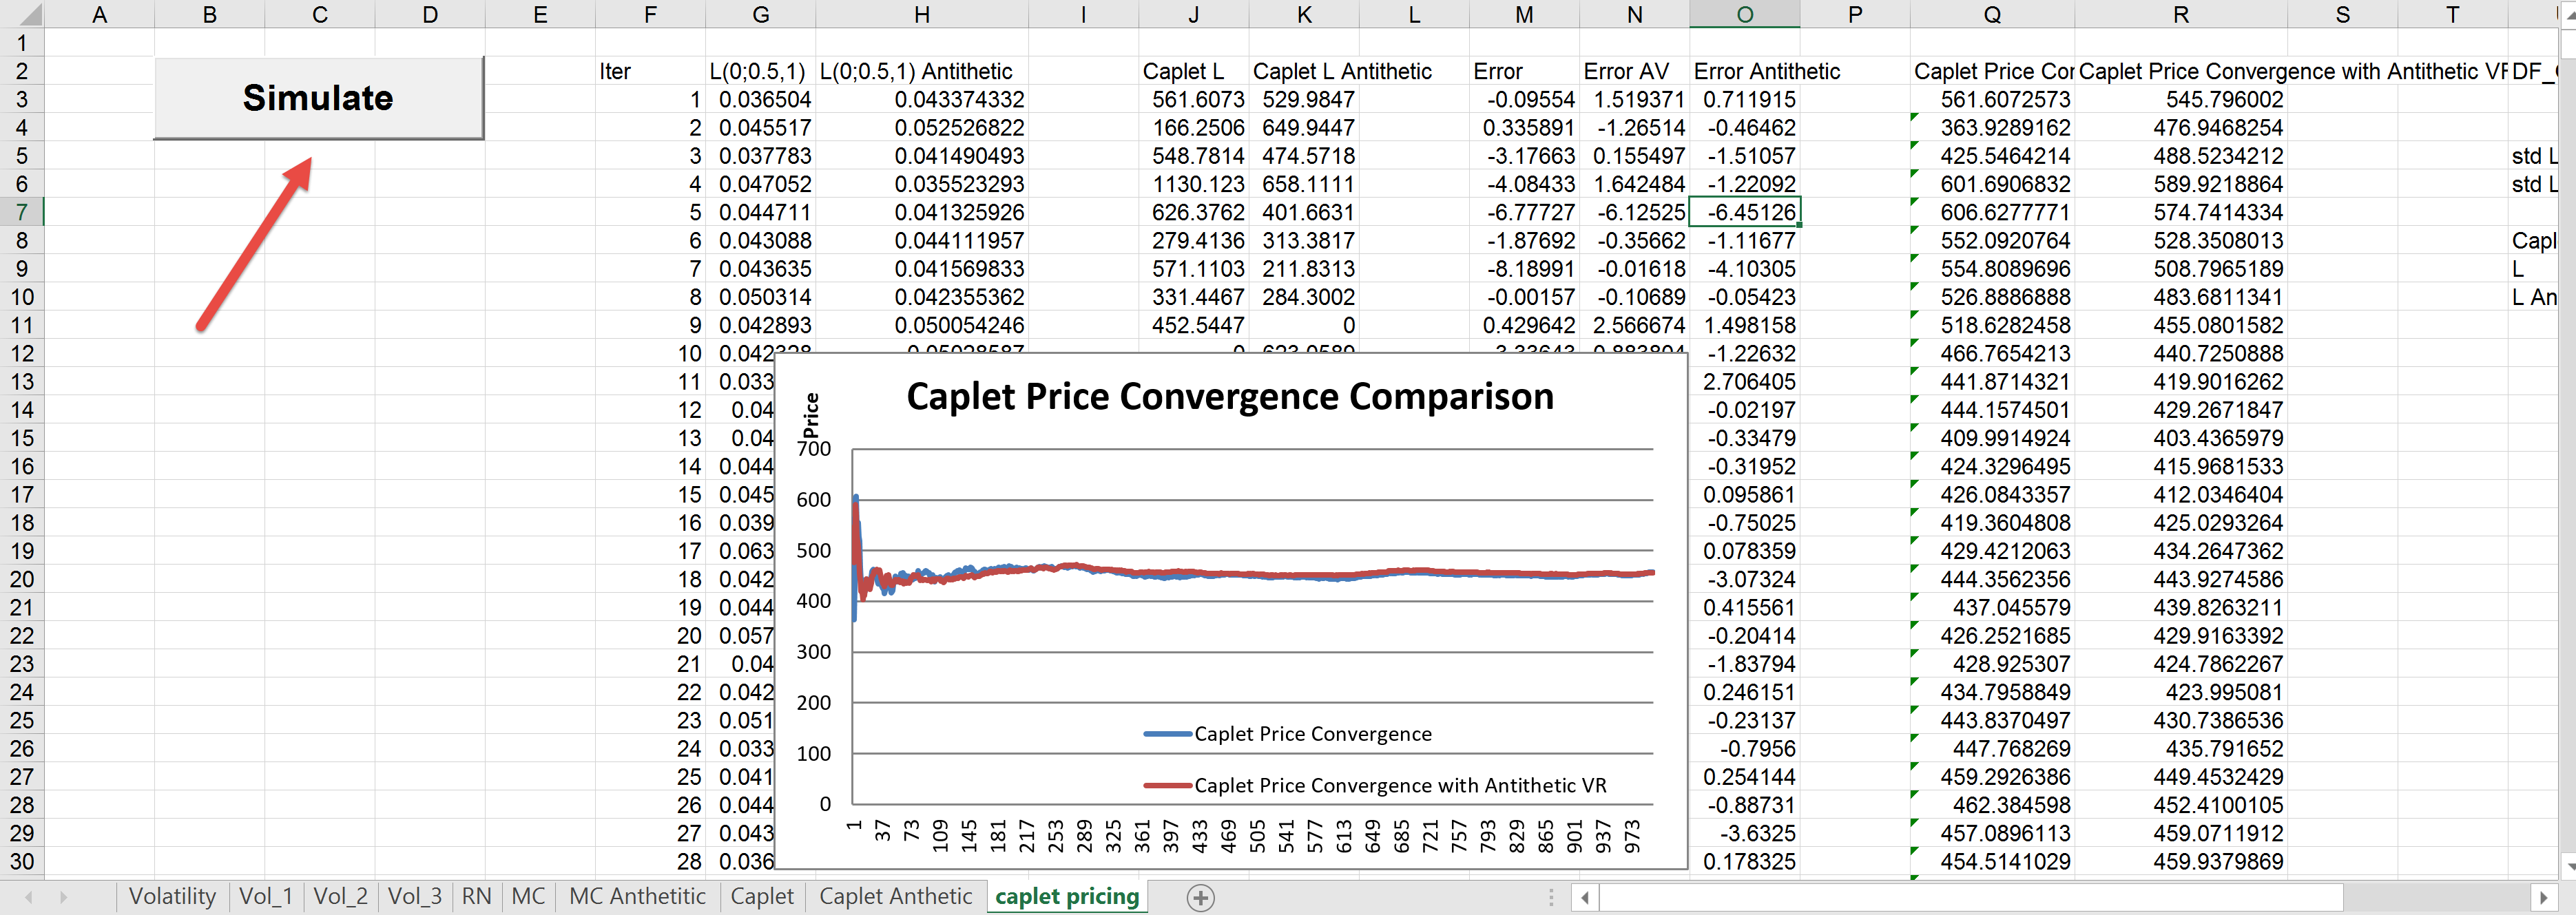
\includegraphics[scale=0.4]{spreadsheet.png}
  \caption{The screen print of the Caplet pricing spreadsheet.}\label{fig::scr_excel}
\end{figure}
\end{center}

Figure~\ref{fig::scr_conv} illustrate the convergence of the Caplet price under regular Monte Carlo simulation and under MC simulation with antithetic variance reduction technique. From the graph, the red line (represents the MC simulation with antithetic VR) seems to have lower estimation variance and faster convergence.

\begin{center}
\begin{figure}
  \centering
  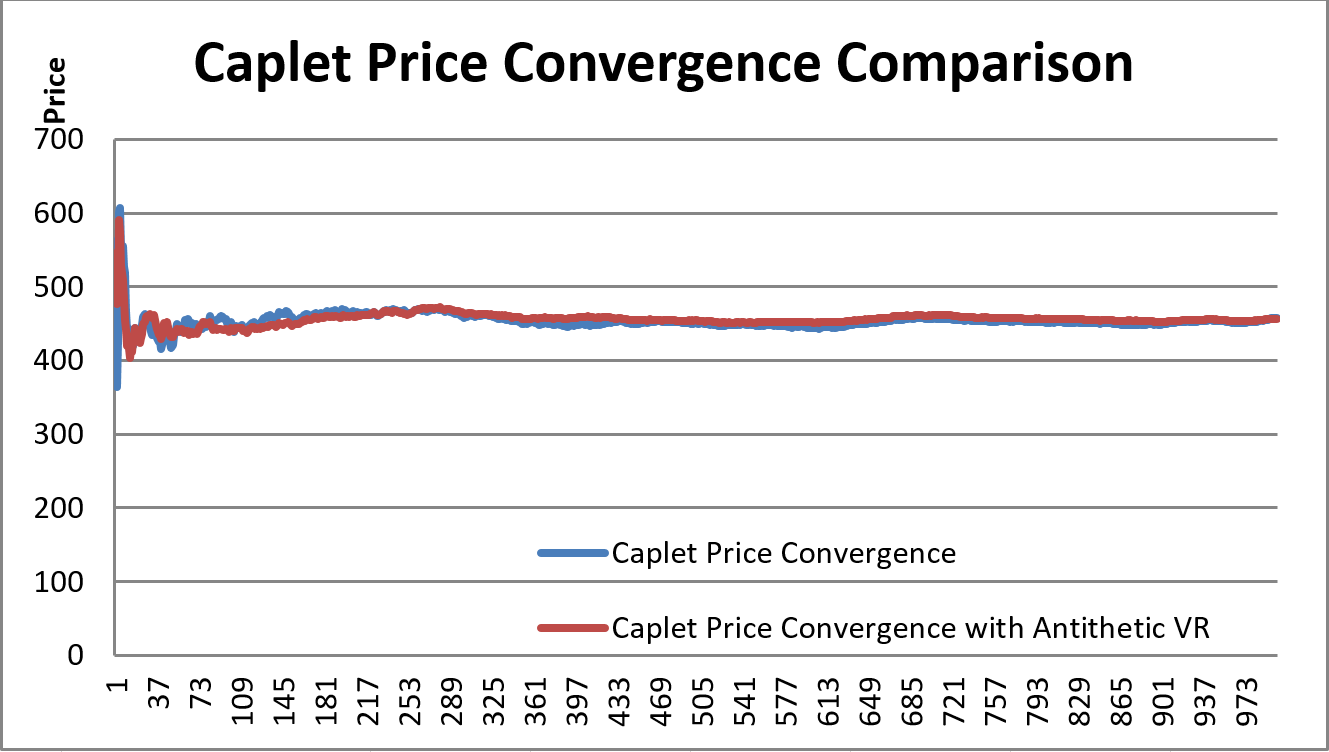
\includegraphics[scale=0.5]{diagram.png}
  \caption{The convergence diagram of Caplet pricing with vs. without antithetic variance reduction.}\label{fig::scr_conv}
\end{figure}
\end{center}

Table~\ref{tbl::numerical_ret} lists the comparison on the convergence of Caplet price between two MC techniques. The MC with antithetic variance reduction has lower standard deviation on the forward rate estimation (10.23 vs. 12.38), and smaller root mean squared error compared to the Black formula pricing.

\begin{table}
  \centering
  \begin{tabular}{|c|c|c|c|} 
  \hline
  % after \\: \hline or \cline{col1-col2} \cline{col3-col4} ...
  MC & Std on Forward Rate & RMSE with Black Formula & Caplet Price \\ \hline
  Without Antithetic VR  & 12.3812 & 0.0713 & 457.3622 \\
  With Antithetic VR & 10.2327 & 0.0520 & 456.7854 \\
  \hline
  \end{tabular}
  \caption{Numerical results comparison on Caplet pricing with and without antithetic variance reduction.}\label{tbl::numerical_ret}
\end{table}

The calculation spreadsheet with VBA and above results is attached to the solution submission.

\end{document} 